\newpage
\section{Instalación de Linux}
En primer lugar, \textbf{si NO queréis instalar Linux}, porque no lo vais a usar para nada más, a parte de las actividades de FDIst, os recomiendo \textbf{leer el apartado \textit{2.1}}, saltaros el resto e ir al punto \textbf{\textit{3.Instalación de una Máquina Virtual en Windows}}.

\subsection{Elección de la distribución}
Existen múltiples distribuciones de Linux, nosotros os haremos una \textbf{lista de recomendaciones basadas en Debian y Arch}, pero podéis descargar la que más os guste:
\begin{itemize}
    \item \textbf{Ubuntu}: Es la más popular y no es casualidad, pues esta distribución se creó para llevar Linux al público en general. Es la más sencilla de usar y la que dispone de un entorno más familiar, por contra, es de las que peor rendimiento tiene.
    \newline Podéis descargar la última versión desde su página oficial: \newline \url{https://ubuntu.com/download/desktop}. 
    
    \item \textbf{Ubuntu Mate}: Una de mis favoritas, pues está pensada para equipos con peores prestaciones que Ubuntu, sin embargo, mantiene ese entorno familiar para los usuarios poco experimentados.
    \newline Podéis descargar la última versión desde su página oficial: \newline \url{https://ubuntu-mate.org/download/}.
    
    \item \textbf{Linux Mint}: Ligero y fácil de usar. Esa es la filosofía que marca a esta distribución, muy recomendada para equipos modestos y para amantes de Windows.
    \newline Podéis descargar la última versión desde su página oficial: \newline \url{https://linuxmint.com/download.php}.
     
    \item \textbf{Manjaro}: Bueno, bonito y gratis, pero no es tan sencillo de instalar como el resto de distribuciones. Si es la primera vez que instaláis Linux os costará, si no, esta distribución os encantará.
    \newline Podéis descargar la última versión desde su página oficial: \newline \url{https://manjaro.org/download/}.
     
    \item \textbf{Raspbian}: No es mala idea tener una Raspberry Pi conectada en casa y hacer ataques desde la FDI, conectado a ella mediante SSH (es lo que hago yo), para ello, os recomendamos el SO, creado exclusivamente para esta plataforma.
    \newline Podéis descargar la última versión desde su página oficial: \newline \url{https://www.raspberrypi.org/downloads/}.
     
    \item \textbf{Debian}: Por qué hablar de distribuciones para Debian, si tenemos el propio Debian. El \textit{sistema operativo universal}, no apto para \textit{noobs}. Realmente, sólo te recomendamos instalar este SO, si tienes experiencia en la plataforma Linux.
    \newline Podéis descargar la última versión desde su página oficial: \newline \url{https://www.debian.org/distrib/netinst}.
   
\end{itemize}

\subsection{Preparación de la unidad de instalación}
Una vez elegida nuestra distribución favorita y descargada la imagen de la misma (.ISO), podremos pasar a instalarla.
\newline\\ Para ello necesitaremos lo siguiente:
\begin{itemize}
    \item Un \textbf{PenDrive} de al menos 8Gb (en algunos casos valdrá con menos capacidad).
    \item La \textbf{ISO} descargada de la distribución que queramos instalar.
    \item El programa \textbf{RUFUS}, para la preparación del PenDrive. 
    \newline Lo podéis descargar desde esta página: \url{https://rufus.ie/}
\end{itemize}

\noindent Preparación de la unidad USB (Advertencia, la unidad se formateará y se perderá toda la información contenida en su interior, por favor, realiza una copia de seguridad de tus archivos):
\begin{enumerate}
    \item Introducimos la unidad USB en el PC donde hayamos descargado la ISO e iniciamos RUFUS.
    \item Pulsamos \textit{SELECCIONAR} y buscamos la el archivo ISO en la página donde lo hayamos guardado.
    \begin{figure}[H]
        \centering
        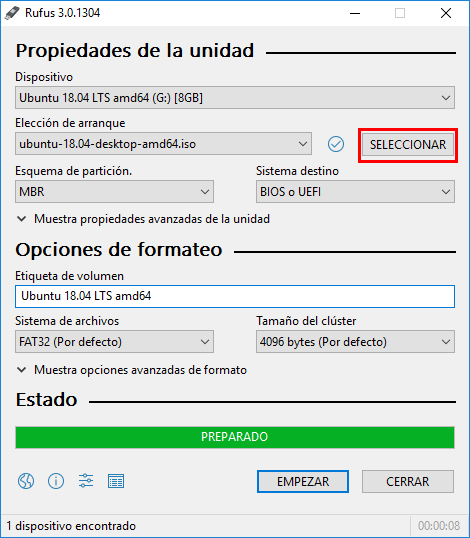
\includegraphics[width= 0.4 \textwidth]{Media/rufus_es_ISO.png}
    \end{figure}
    \newpage
    \item Pulsamos \textit{EMPEZAR} y esperamos al que el programa prepare la unidad. Una vez finalizado, \textbf{extraemos el pendrive con srguridad} y listo.
    \begin{figure}[H]
        \centering
        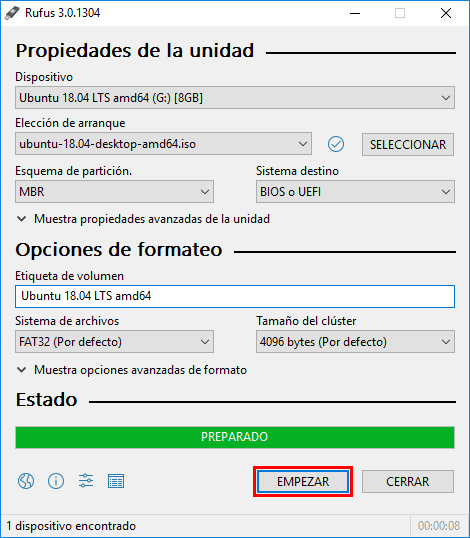
\includegraphics[width= 0.4 \textwidth]{Media/rufus_es_empezar.png}
    \end{figure}
\end{enumerate}

\subsection{Arrancar el instalador del sistema}
\begin{enumerate}
    \item Introducimos la unidad de instalación USB que hemos preparado anteriormente en el ordenador en el que queramos instalar el SO.
    \item Si en la BIOS no tenemos seleccionado que la unidad de arranque primaria sea el USB, pulsaremos rápidamente F12 hasta que nos aparezca el \textit{"Boot Menu"} (en algunas placas base puede variar, consultar en la web oficial del fabricante).
    \item Seleccionamos el USB como unidad de arranque y se iniciará el instalador de la distribución de Linux elegida.
    \begin{figure}[H]
        \centering
        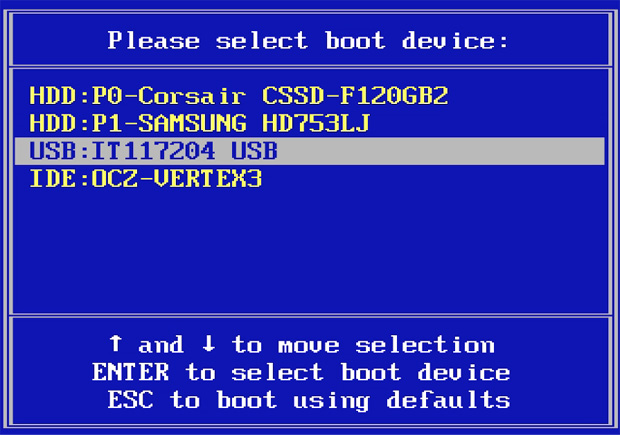
\includegraphics[width= 0.5 \textwidth]{Media/boot-menu-formatear-pc.jpg}
    \end{figure}
\end{enumerate}

\subsection{Opciones de instalación}
    \subsubsection{Idioma} 
    Seleccionamos el idioma que deseemos para el sistema y pulsamos en \textit{'Continuar'}.
     \begin{figure}[H]
        \centering
        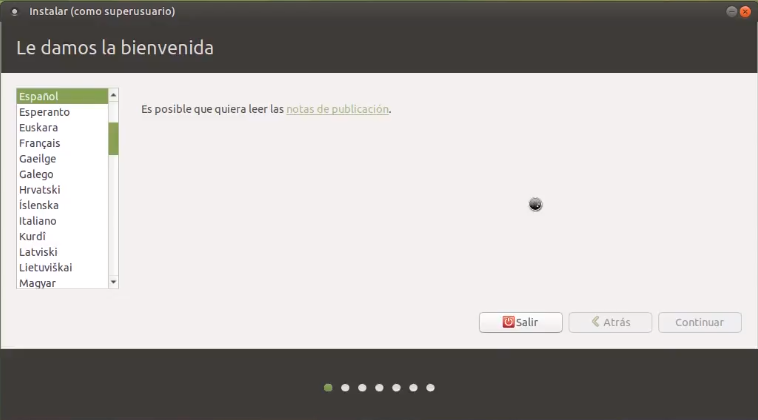
\includegraphics[width= 0.7 \textwidth]{Media/umate1.png}
    \end{figure}
    \subsubsection{Distribución de teclado}
    Seleccionamos la distribución de teclado que queramos (aseguraos de que la distribución seleccionada es la \textbf{ESPAÑOLA}, si no luego tendréis muchos problemas a la hora de escribir) y pulsamos en \textit{'Continuar'}.
     \begin{figure}[H]
        \centering
        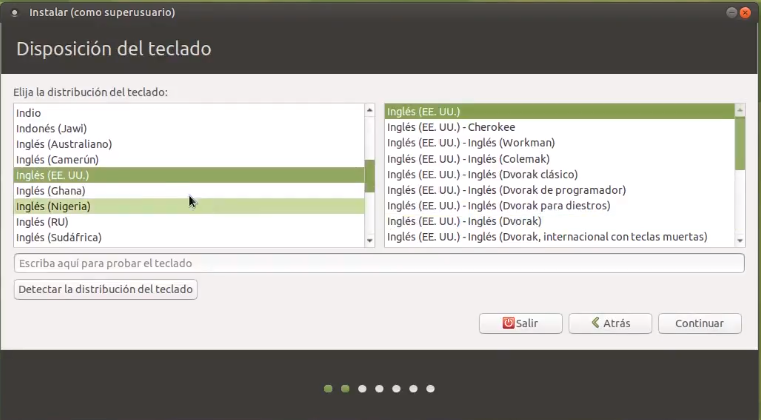
\includegraphics[width= 0.7 \textwidth]{Media/umate2.png}
    \end{figure}

\newpage    
\subsubsection{Programas y drivers} 
    A continuación nos aparecerán una serie de opciones:
     \begin{figure}[H]
        \centering
        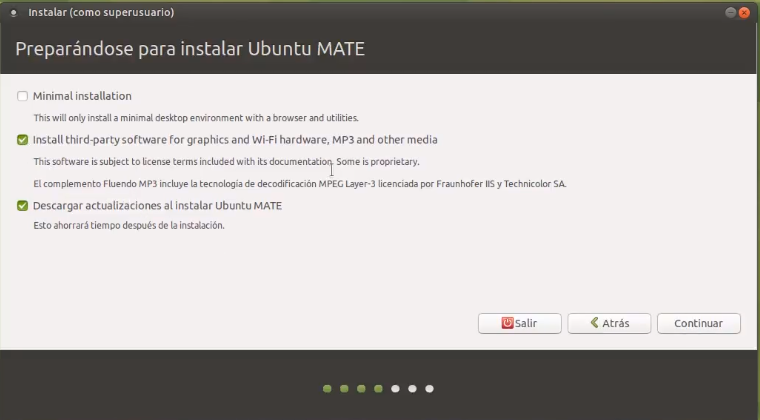
\includegraphics[width= 0.7 \textwidth]{Media/umate3.png}
    \end{figure}
    \begin{itemize}
        \item \textbf{Instalación mínima}: esta opción es recomendable si vamos a instalar Linux junto con Windows y queremos dedicar poco espacio a la partición de Linux. Al seleccionar esta opción, se nos instalarán los programas básicos del sistema y nos ahorraremos espacio, pues no se instalarán herramientas como \textit{LibreOffice} que no utilizaremos.
        \item \textbf{Instalación de software de terceros}: Importante marcar esta opción, pues descargará e instalará drivers que puedan necesitar componentes de nuestro hardware, como los de la tarjeta de red inalámbrica o nuestra tarjeta gráfica.
        \item \textbf{Descargar actualizaciones al instalar}: Opcional, pero recomendado marcarlo, la instalación tardará unos minutos más, pero luego no tendremos que buscar la última actualización manualmente.
    \end{itemize}
   
    Cuando hayamos seleccionado las opciones que deseemos, pulsamos en \textit{'Continuar'}.
    
\subsubsection{Tipo de instalación}
Ahora es el momento de decidir si queremos instalar Linux junto con Windows, o por el contrario, formatear la unidad e instalar únicamente Linux (borrando Windows de forma permanente.
\begin{figure}[H]
        \centering
        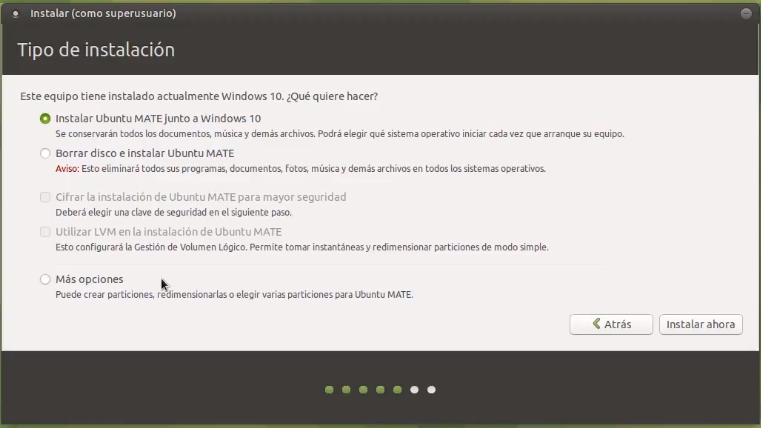
\includegraphics[width= 0.7 \textwidth]{Media/umate4.png}
\end{figure}

\begin{itemize}
    \item \textbf{Instalar Linux junto a Windows}: Esta opción creará automáticamente una partición en nuestro disco duro, donde instalará la distribución de Linux, conservando Windows. Al arrancar el equipo, el GRUB de Linux nos permitirá elegir que sistema arrancar (por defecto pondrá Linux, pero más tarde, podremos modificar el orden de arranque si por defecto queremos poner Windows).
    \item \textbf{Borrar disco e instalar Linux}: Formateará por completo la unidad, eliminará Windows y todos los archivos que contenga, perderemos la licencia del SO.
    \newline \textit{Si seleccionamos esta opción, se nos habilitarán las siguientes opciones}:
    \item \textbf{Cifrar la instalación de Linux para mayor seguridad}: Esto hará que los datos contenidos en el disco sean cifrados, la instalación tardará un poco más y tendrá un impacto en el rendimiento del equipo, por tanto, si tenemos un ordenador con componentes de baja calidad, no es recomendable. Por el contrario, si queremos proteger muy bien nuestros archivos, entonces es recomendable seleccionar esta opción.
    \item \textbf{Utilizar LVM}: Esto no es más que un sistema que administración de discos, es recomendable seleccionar esta opción, pues en un futuro puede que queramos volver a instalar Windows o otra distribución de Linux junto con la actual.
\end{itemize}
Por otra parte, si queremos instalar Linux junto con Windows, pero queremos seleccionar nosotros mismos el espacio que se le dedica a cada Sistema Operativo, seleccionaremos la siguiente opción:
\begin{itemize}
    \item \textbf{Más opciones}: Nos permitirá crear la partición de Linux con el tamaño que queramos, ajustando así, cuánto espacio del disco le dejamos a Windows. Es recomendable usar al menos 30GB para la mayoría de distribuciones de Linux, aunque con menos podrían funcionar.
\end{itemize}
Por último, pulsamos en \textit{'Instalar ahora'}.

\subsubsection{Zona horaria}
Seleccionaremos la región donde nos encontremos, en nuestro caso, Madrid. Y pulsamos en \textit{'Continuar'}.
\begin{figure}[H]
        \centering
        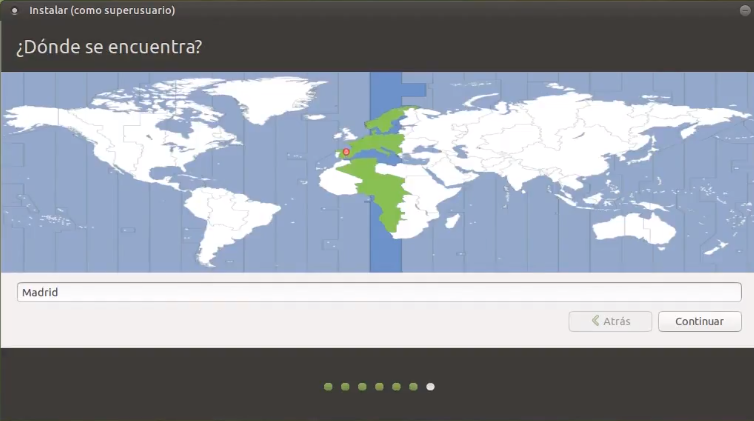
\includegraphics[width= 0.7 \textwidth]{Media/umate5.png}
\end{figure}

\subsection{Usuario y contraseña}
Por último, le asignaremos un nombre al equipo, crearemos el usuario con el nombre que queramos e creamos una nueva contraseña. Si queremos podemos seleccionar la opción de \textit{'Iniciar sesión automáticamente'}, para que no nos pida nuestra contraseña al iniciar nuestro ordenador (más cómodo, pero mucho más inseguro). 
\newline Pulsamos en \textit{'Continuar'} y comenzará la instalación.
\begin{figure}[H]
        \centering
        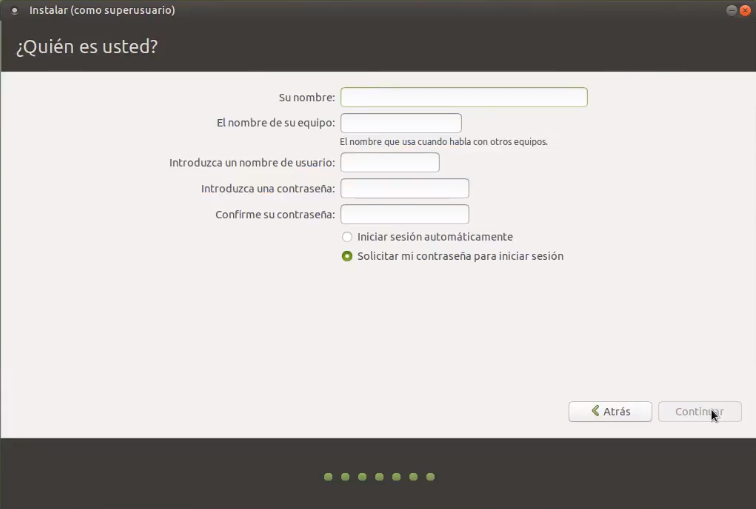
\includegraphics[width= 0.7 \textwidth]{Media/umate6.png}
\end{figure}

\newpage
\subsection{Finalizar la instalación}
Cuando la instalación finalice, nos aparecerá un nuevo cuadro de diálogo, en el que pulsaremos en \textit{'Reiniciar ahora'} y ya podremos comenzar a usar nuestra distribución de Linux.
\begin{figure}[H]
        \centering
        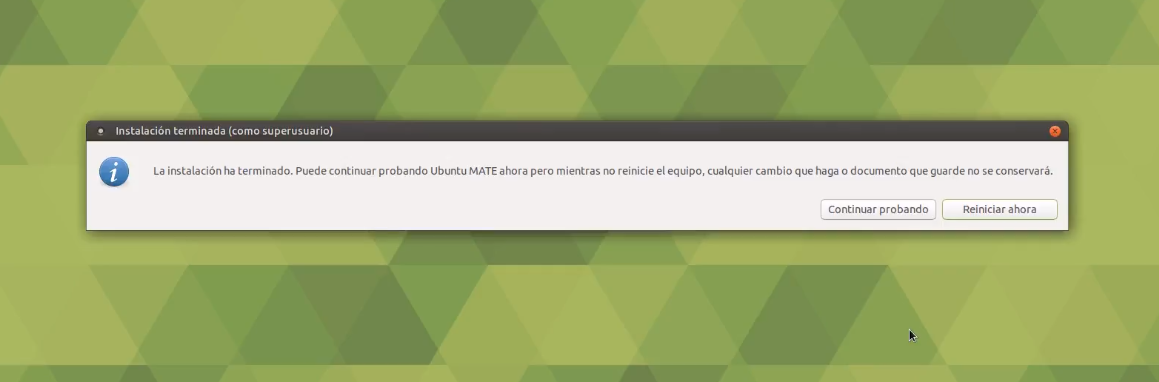
\includegraphics[width= 0.7 \textwidth]{Media/umate7.png}
\end{figure}

\subsubsection{Poner Windows como primera opción del GRUB}
Como habremos observado, al reiniciar el equipo (si hemos instalado Linux junto con Windows, nos aparecerá la ventana en la que nos permite escoger que SO iniciar.
\newline Por defecto viene seleccionada la distrubución de Linux que hayamos instalado y hay una cuenta atrás que iniciará está automáticamente, a no ser que toquemos alguna flecha del teclado para seleccionar otra opción.
\begin{figure}[H]
        \centering
        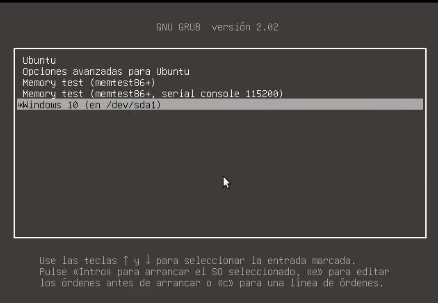
\includegraphics[width= 0.7 \textwidth]{Media/grub.png}
\end{figure}
\newline A continuación os explico cómo poner Windows por defecto:
\begin{enumerate}
    \item Abriremos una terminal desde nuestra distribución de Linux y escribiremos el siguiente comando: \textbf{sudo nano /boot/grub/grub.cfg}
    \item Se nos abrirá un documento editable como este:
    \begin{figure}[H]
        \centering
        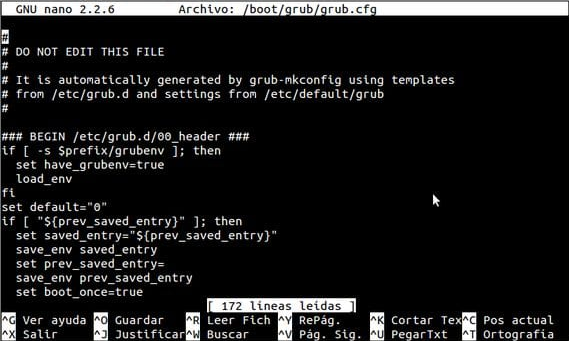
\includegraphics[width= 0.7 \textwidth]{Media/grubload.png}
    \end{figure}
    En donde tendremos que modificar sólo la linea \textbf{\verb=set default='0'}. Cambiando el '0' por el '4', que es el número que, en mi caso, corresponde a la partición de Windows que esta instalada junto a tu sistema Linux.
    \item Hecho esto, pulsamos 'CTRL+X' para salir, pulsamos la tecla 'S' para guardar y a continuación la tecla 'ENTER' para confirmar.
\end{enumerate}
Y listo, la próxima vez que iniciemos el equipo, Windows será la opción por defecto.